\ifdefined\withimages
	\newpage
	\tikz[remember picture,overlay] \node[opacity=1,inner sep=0pt] at (current page.center){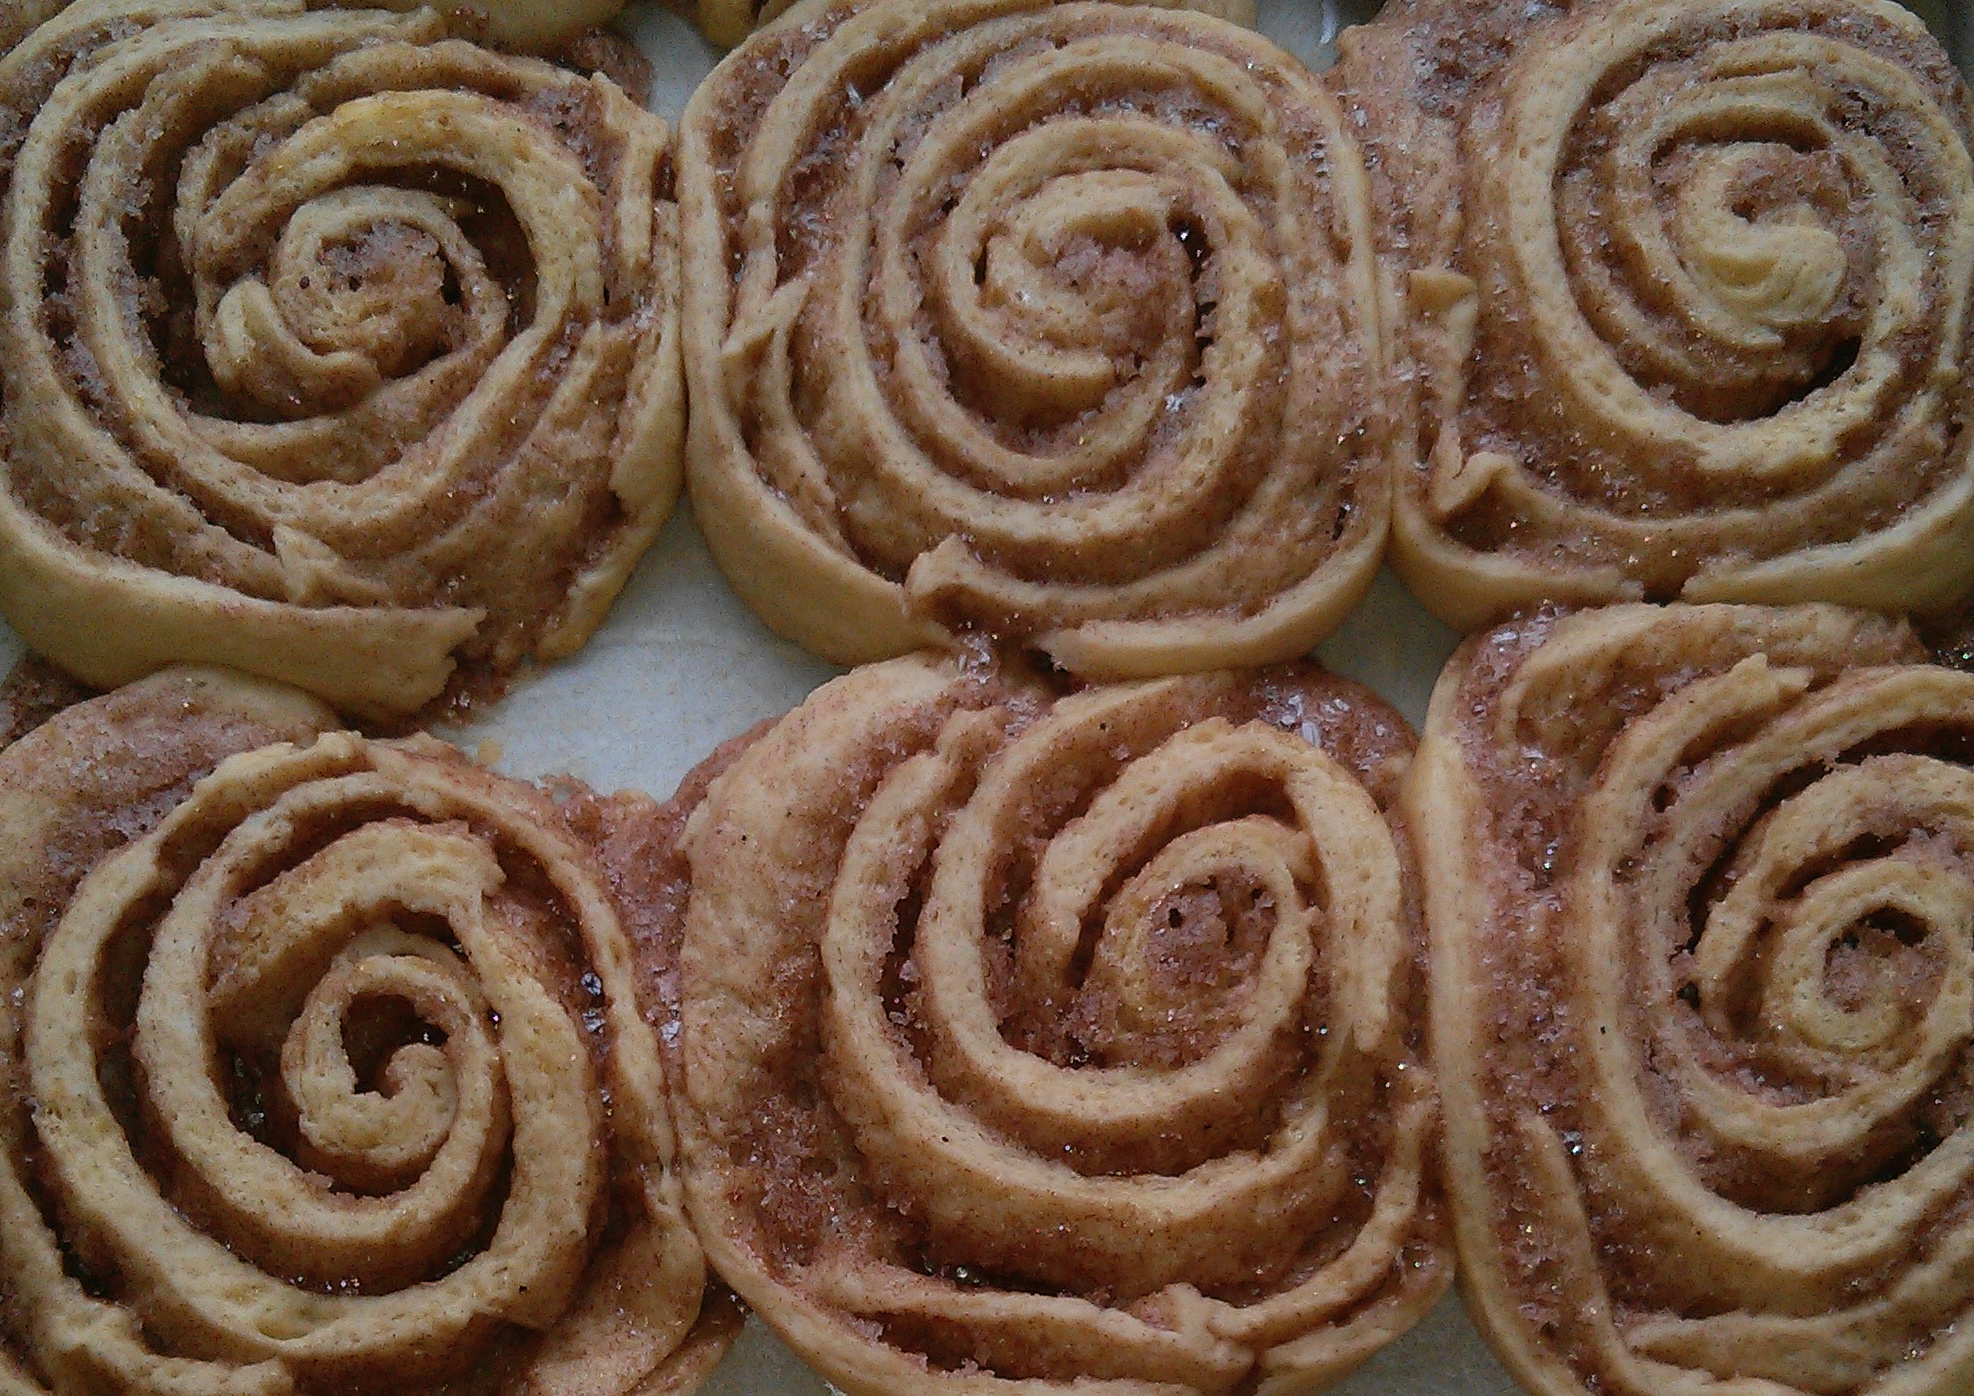
\includegraphics[width=\paperwidth,height=\paperheight]{./bilder/zimtschnecken_ratio.jpg}};
\fi

\begin{recipe}[]{Zimtschnecken} %Josi
	\timerecipe[Minuten]{ca. 120} %mit [EINHEIT]
	
	\personcount[Blech]{1} % mit[ART]
	\ingredient{500g Mehl}
	\ingredient{50g Hefe}
	\ingredient{250ml lauwarme Milch}
	\ingredient{270g weiche Butter}
	\ingredient{250g Zucker}
	\ingredient{0,5 TL Kardamom}
	\ingredient{2 EL Zimt}
	\ingredient{0,5 TL Salz}

\step
Die \textbf{500g Mehl} in eine Schüssel geben in einer Kuhle \textbf{250ml lauwarme Milch} und \textbf{50g Hefe} vermischen und ca. 10 min gehen lassen. 

\step
Zusammen mit \textbf{70g weiche Butter}, \textbf{0,5 TL Kardamom} und \textbf{0,5 TL Salz} zu einem Teig verkneten und 40 min gehen lassen.

\step
In der Zwischenzeit für die Füllung \textbf{200g weiche Butter}, \textbf{200g Zucker} mit \textbf{2 EL Zimt} cremig schlagen.

\step
Teig nocheinmal kräftig kneten, in zwei Teile teilen, jeweils ca. 30 cm breit ausrollen und mit der Füllungsmasse bestreichen. Die beiden Teige aufeinanderlegen und aufrollen.

\step
Die Teigrolle in ca. 3 cm breite Scheiben schneiden und diese auf einem Blech mit auslegen. Vor dem Backen nochmals 20 min gehen lassen. 

\step
Backofen vorheizen. Auf mittlerer Schiene 10 min bei 200°C und dann nochmals ca. 15 min bei 180°C backen. 

% Seite mit Bild nach dem Rezept
%\graphic{./bilder/zimtschnecken.jpg}

\tippbox{\textbf{Tipp:} Seiten der Zimtrollen vor dem Backen noch mit Eigelb einpinseln.} % Tipp in extra Rahmen

\end{recipe}

% background Image
%\tikz[remember picture,overlay] \node[opacity=0.3,inner sep=0pt] at (current page.center){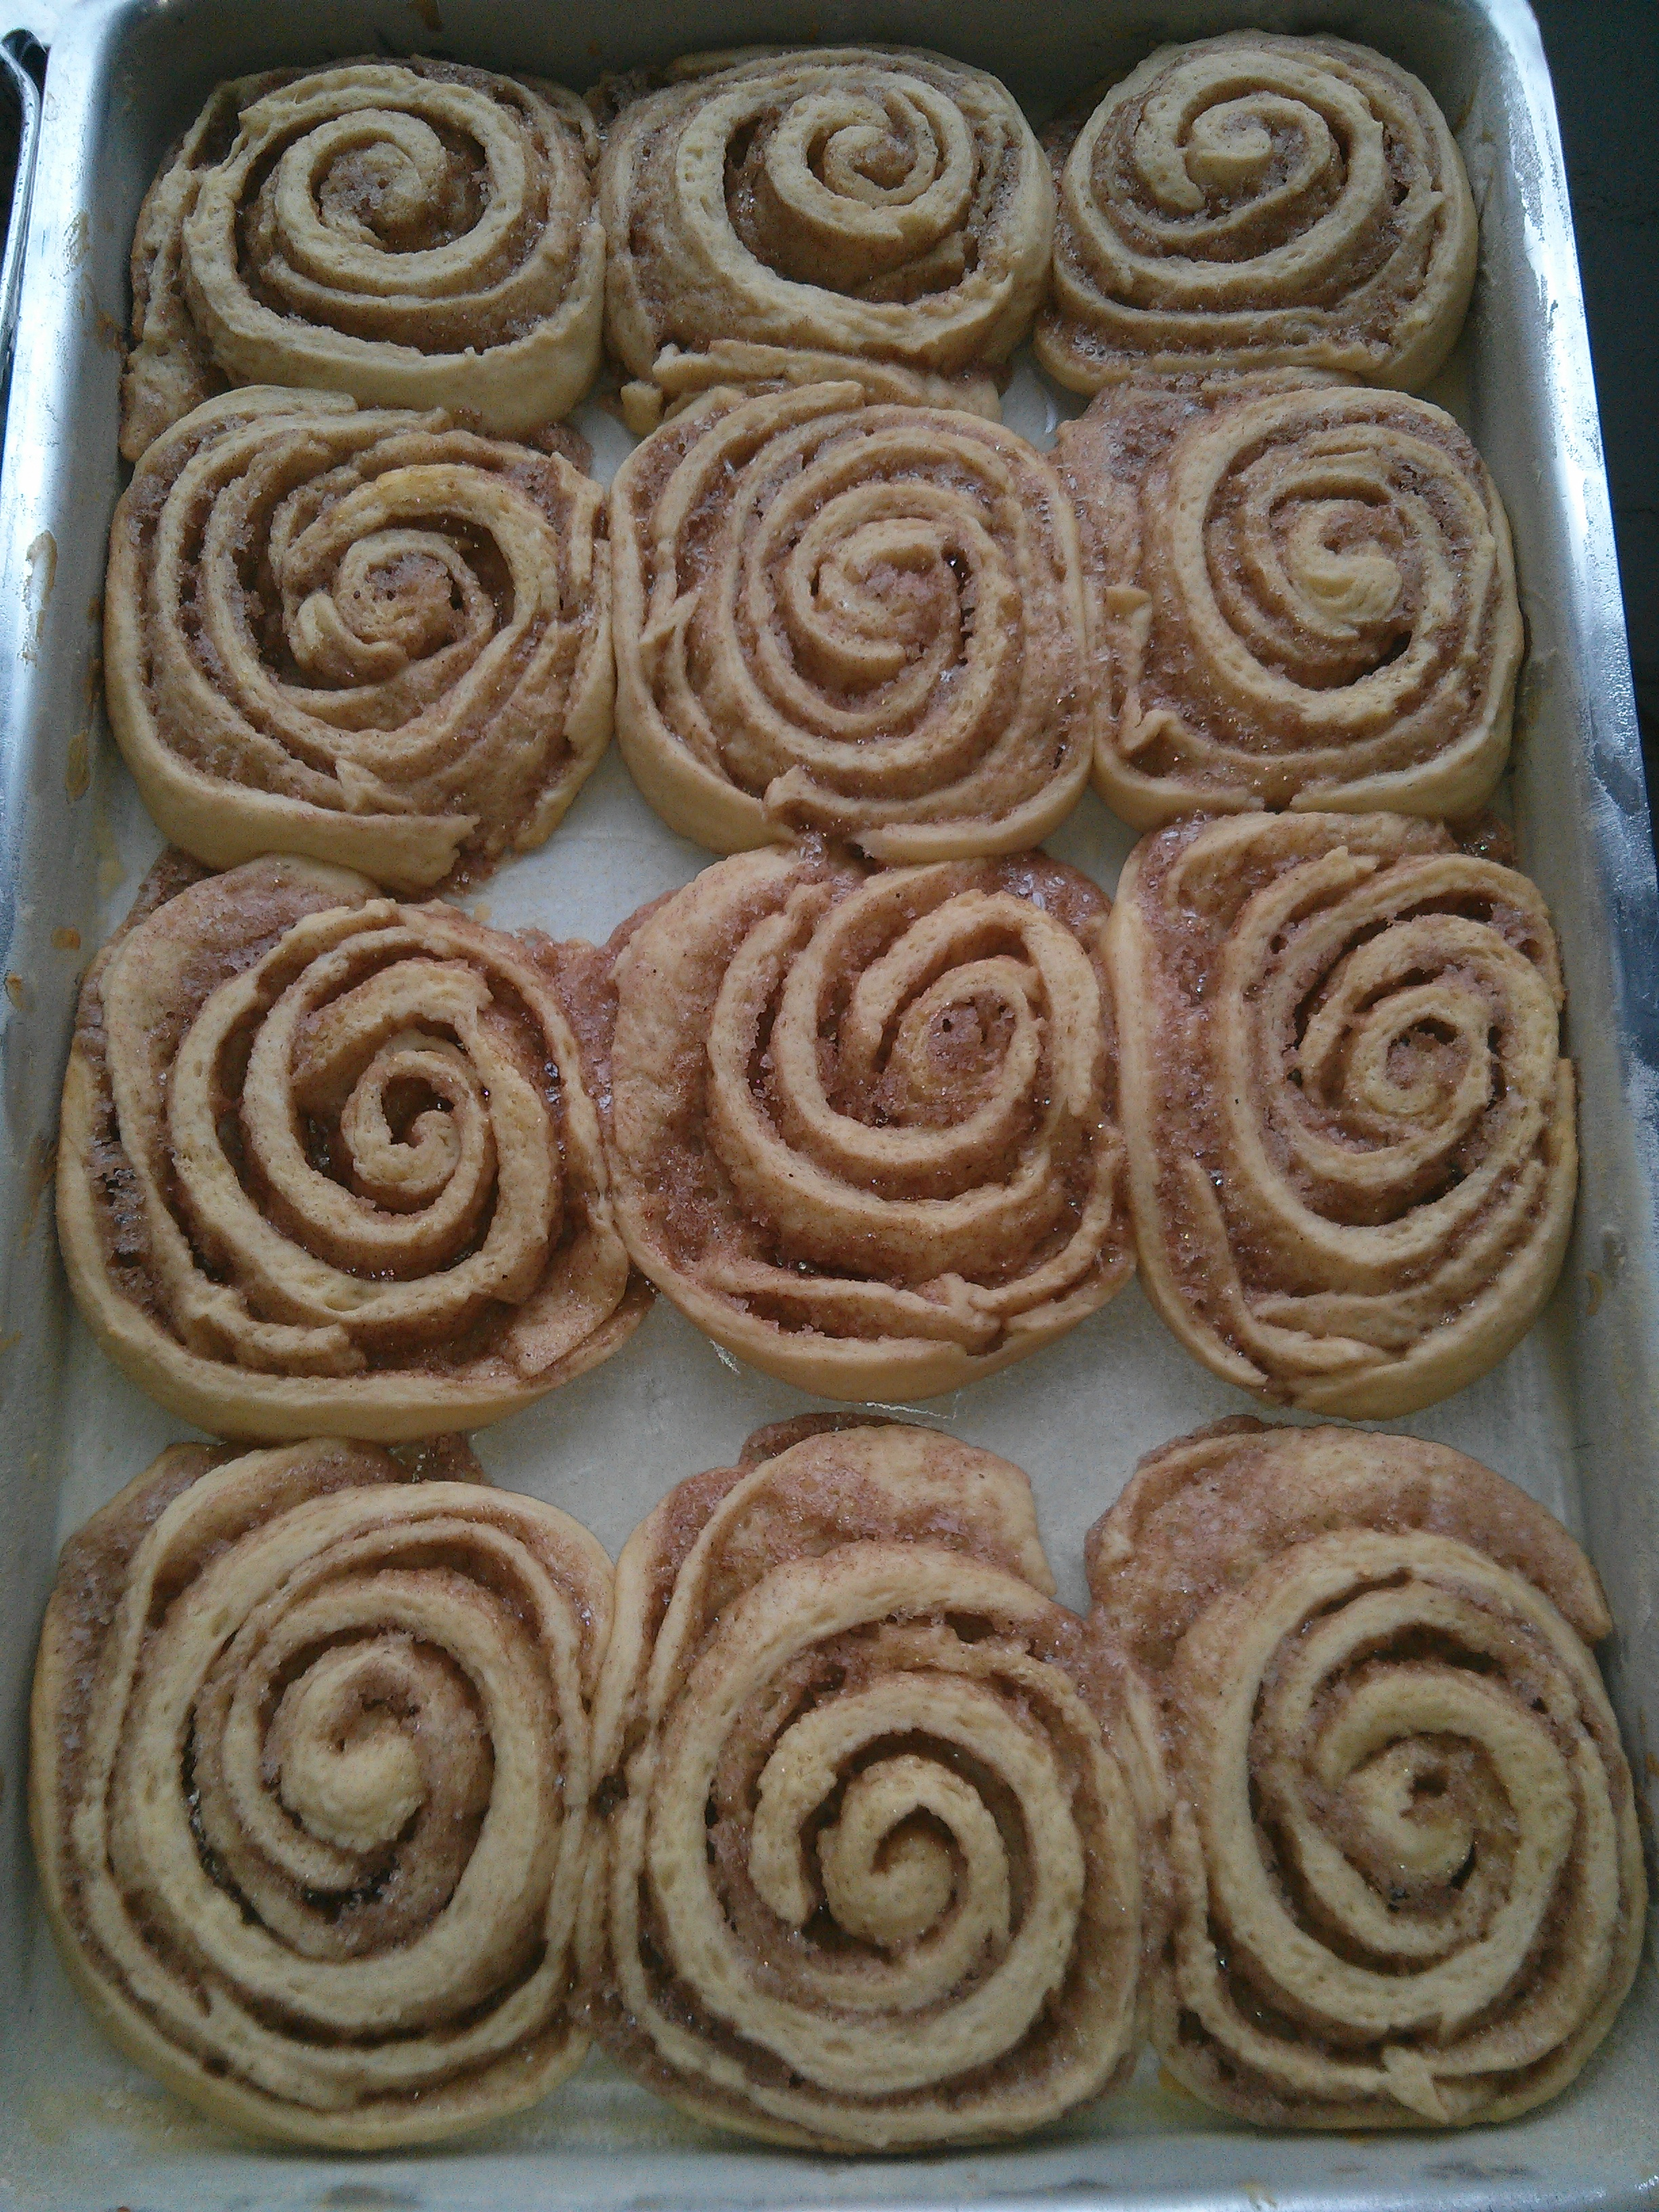
\includegraphics[width=\paperwidth,height=\paperheight]{./bilder/zimtschnecken.jpg}};
